%定义文档类型和基本的页面设置
\documentclass[12pt,a4paper]{article}

%加载要用到的宏包
\usepackage[utf8]{inputenc}
\usepackage{amsmath}
\usepackage{amsfonts}
\usepackage{amssymb}
\usepackage{amsthm}
\usepackage{bussproofs}
\usepackage{tikz}
\usepackage{geometry}   %设置页边距的宏包

\geometry{left=1cm,right=1cm,top=2.5cm,bottom=2.5cm}

%自定义环境
\theoremstyle{plain}
\newtheorem{exercise}{Exercise}

%文档的标题
\title{Homework 4}

%文档的作者
\author{\\
}

%文档的日期
\date{Deadline: 23:59, November 1st, 2018}

%文档内容开始
\begin{document}

%打出文档的标题、作者、日期等信息
\maketitle

Please do Exercises 3.1.1(d), 3.1.3, 3.2.3, 3.2.4 and 3.2.5 in the textbook and compare your solutions to those at the end of the book.

You do NOT need to hand in your solutions to the above exercises.

\ \\
\textbf{Exercise 7 in Homework 3.}
\textit{Please solve (a) and (c) in Exercise 2.6.2 in the textbook:}

\textit{Find natural deduction proofs for the following sequents (all of which need (RAA)):}
%
\begin{enumerate}

\item[(a)] \textit{$\{ ( ( \neg \psi ) \rightarrow ( \neg \phi ) ) \} \vdash ( \phi \rightarrow \psi )$.}

\item[(c)] \textit{$\vdash ( \phi \rightarrow ( ( \neg \phi ) \rightarrow \psi ) )$.}

\end{enumerate}

\begin{proof}[Solution]\
    \begin{enumerate}
        \item[(a)]\
            \begin{prooftree}
                 \AxiomC{$[\phi]^2$}
                 \AxiomC{$[\neg \psi]^1$}
                 \AxiomC{$\neg \psi \to \neg \phi$}
                 \RightLabel{$(\to E)$}
                 \BinaryInfC{$\neg \phi$}
                 \RightLabel{$(\neg E)$}
                 \BinaryInfC{$\bot$}
                 \RightLabel{$(RAA),1$}
                 \UnaryInfC{$\psi$}
                 \RightLabel{$(\to I),2$}
                 \UnaryInfC{$\phi \to \psi$}
            \end{prooftree}
        \item[(c)]\
              \begin{prooftree}
                \AxiomC{$[\neg \psi]^1$}
                \AxiomC{$[\phi]^3$}
                \RightLabel{$(\to I)$}
                \UnaryInfC{$\neg \psi \to \phi$}
                \RightLabel{$(\to E)$}
                \BinaryInfC{$\phi$}
                \AxiomC{$[\neg \psi]^1$}
                \AxiomC{$[\neg \phi]^2$}
                \RightLabel{$(\to I)$}
                \UnaryInfC{$\neg \psi \to \neg \phi$}
                \RightLabel{$(\to E)$}
                \BinaryInfC{$\neg \phi$}
                \RightLabel{$(\neg E)$}
                \BinaryInfC{$\bot$}
                \RightLabel{$(RAA),1$}
                \UnaryInfC{$\psi$}
                \RightLabel{$(\to I),2$}
                \UnaryInfC{$\neg \phi \to \psi$}
                \RightLabel{$(\to I),3$}
                \UnaryInfC{$\phi \to (\neg \phi \to \psi)$}
            \end{prooftree}
         
    \end{enumerate}
\end{proof}

\ \\
\ \\
\textbf{Exercise 8 in Homework 3.}
\textit{Please solve (b) and (c) in Exercise 2.7.1 in the textbook:}

\textit{Find natural deduction proofs of the following sequents (none of which need ($\vee$E)):}
%
\begin{enumerate}

\item[(b)] \textit{$\{ ( \neg ( \phi \vee \psi ) ) \} \vdash ( ( \neg \phi ) \wedge ( \neg \psi ) )$.}

\item[(c)] \textit{$\vdash ( \phi \rightarrow \psi ) \rightarrow ( ( \neg \phi ) \vee \psi )$.}

\end{enumerate}

\begin{proof}[Solution]\
    \begin{enumerate}
        \item[(b)]\
            \begin{prooftree}
                \AxiomC{$[\phi]^1$}
                \RightLabel{$(\vee I)$}
                \UnaryInfC{$\phi \vee \psi$}
                \AxiomC{$\neg (\phi \vee \psi)$}
                \RightLabel{$(\neg E)$}
                \BinaryInfC{$\bot$}
                \RightLabel{$(RAA),1$}
                \UnaryInfC{$\neg \phi$}
                \AxiomC{$[\psi]^2$}
                \RightLabel{$(\vee I)$}
                \UnaryInfC{$\phi \vee \psi$}
                \AxiomC{$\neg (\phi \vee \psi)$}
                \RightLabel{$(\neg E)$}
                \BinaryInfC{$\bot$}
                \RightLabel{$(RAA),2$}
                \UnaryInfC{$\neg \psi$}
                \RightLabel{$(\vee I)$}
                \BinaryInfC{$( ( \neg \phi ) \wedge ( \neg \psi ) )$}
            \end{prooftree}    
        \item[(c)]\
            \begin{prooftree}
                \AxiomC{$[\neg \phi]^1$}
                \RightLabel{$(\vee I)$}
                \UnaryInfC{$\neg \phi \vee \psi$}
                \AxiomC{$[\neg (\neg \phi \vee \psi)]^3$}
                \RightLabel{$(\to E)$}
                \BinaryInfC{$\bot$}
                \RightLabel{$(RAA),1$}
                \UnaryInfC{$\phi$}
                \AxiomC{$[\phi]^2$}
                \AxiomC{$[\phi \to \psi]^4$}
                \RightLabel{$(\to E)$}
                \BinaryInfC{$\psi$}
                \RightLabel{$(\vee I),2$}
                \UnaryInfC{$\neg \phi \vee \psi$}
                \AxiomC{$[\neg (\neg \phi \vee \psi)]^3$}
                \RightLabel{$(\to E)$}
                \BinaryInfC{$\bot$}
                \RightLabel{$(RAA),1$}
                \UnaryInfC{$\neg \phi$}
                \RightLabel{$(\to E)$}
                \BinaryInfC{$\bot$}
                \RightLabel{$(RAA),3$}
                \UnaryInfC{$\neg \phi \vee \psi$}
                \RightLabel{$(\to I),4$}
                \UnaryInfC{$( \phi \rightarrow \psi ) \rightarrow ( ( \neg \phi ) \vee \psi )$}
            \end{prooftree}
            
    \end{enumerate}
\end{proof}

\ \\
\ \\
\textbf{Exercise 9 in Homework 3.}
\textit{Please solve (a) - (e) in Exercise 2.7.2 in the textbook:}

\textit{Find natural deduction proofs of the following sequents (These need ($\vee$E)):}
%
\begin{enumerate}

\item[(a)] \textit{$\{ ( \phi \vee \psi) \} \vdash (\psi \vee \phi )$}.

\item[(b)] \textit{$\{ ( \phi \vee \psi ), ( \phi \rightarrow \chi ), (\psi \rightarrow \chi ) \} \vdash \chi$.}

\item[(c)] \textit{$\{ ( \phi \vee \psi ), ( \neg \phi) \} \vdash \psi$.}

\item[(d)] \textit{$\{ (( \neg \phi) \wedge ( \neg \psi )) \} \vdash ( \neg (\phi \vee \psi ))$.}

\item[(e)] \textit{$\{ (\phi \wedge \psi ) \} \vdash ( \neg (( \neg \phi) \vee (  \neg \psi )))$.}

\end{enumerate}

\begin{proof}[Solution]\
    \begin{enumerate}
        \item[(a)]\
            \begin{prooftree}
                \AxiomC{$\phi \vee \psi$}
                \AxiomC{$[\phi]^1$}
                \RightLabel{$(\vee I)$}
                \UnaryInfC{$\psi \vee \phi$}
                \AxiomC{$[\psi]^1$}
                \RightLabel{$(\vee I)$}
                \UnaryInfC{$\psi \vee \phi$}
                \RightLabel{$(\vee E),1$}
                \TrinaryInfC{$\psi \vee \phi$}
            \end{prooftree}
        \item[(b)]\
            \begin{prooftree}
                \AxiomC{$\phi \vee \psi$}
                \AxiomC{$[\phi]^1$}
                \AxiomC{$\phi \to \psi$}
                \RightLabel{$(\vee I)$}
                \BinaryInfC{$\chi$}
                \AxiomC{$[\psi]^1$}
                \AxiomC{$\psi \to \chi$}
                \RightLabel{$(\vee I)$}
                \BinaryInfC{$\chi$}
                \RightLabel{$(\vee E),1$}
                \TrinaryInfC{$\chi$}
            \end{prooftree}
        \item[(c)]\ 
            \begin{prooftree}
                \AxiomC{$\phi \vee \psi$}
                \AxiomC{$[\phi]^2$}
                \AxiomC{$\neg \phi$}
                \RightLabel{$(RAA),1$}
                \BinaryInfC{$\psi$}
                \AxiomC{$[\psi]^2$}
                \RightLabel{$(\vee E),2$}
                \TrinaryInfC{$\psi$}
            \end{prooftree}
        \item[(d)]\ 
            \begin{prooftree}
                \AxiomC{$[\phi \vee \psi]^2$}
                \AxiomC{$[\phi]^1$}
                \AxiomC{$(( \neg \phi) \wedge ( \neg \psi ))$}
                \RightLabel{$(\wedge E)$}
                \UnaryInfC{$\neg \phi$}
                \RightLabel{$(\neg E)$}
                \BinaryInfC{$\bot$}
                \AxiomC{$[\psi]^1$}
                \AxiomC{$(( \neg \phi) \wedge ( \neg \psi ))$}
                \RightLabel{$(\wedge E)$}
                \UnaryInfC{$\neg \psi$}
                \RightLabel{$(\neg E)$}
                \BinaryInfC{$\bot$}
                \RightLabel{$(\vee E),1$}
                \TrinaryInfC{$\bot$}
                \RightLabel{$(\neg I),2$}
                \UnaryInfC{$\neg (\phi \to \psi)$}
            \end{prooftree}
        \item[(e)]\ 
            \begin{prooftree}
                \AxiomC{$[\neg \phi \vee \neg \psi]^2$}
                \AxiomC{$\phi \wedge \psi$}
                \RightLabel{$(\wedge E)$}
                \UnaryInfC{$\phi$}
                \AxiomC{$[\neg \phi]^1$}
                \RightLabel{$(\neg E)$}
                \BinaryInfC{$\bot$}
                \AxiomC{$\phi \wedge \psi$}
                \RightLabel{$(\wedge E)$}
                \UnaryInfC{$\psi$}
                \AxiomC{$[\neg \psi]^1$}
                \RightLabel{$(\neg E)$}
                \BinaryInfC{$\bot$}
                \RightLabel{$(\vee E),1$}
                \TrinaryInfC{$\bot$}
                \RightLabel{$(\neg I),2$}
                \UnaryInfC{$\neg (\neg \phi \vee \neg \psi)$}
            \end{prooftree}
    \end{enumerate}
\end{proof}

\ \\
\begin{exercise}
Please solve Exercise 3.1.2 in the textbook:

Find the associated formula of each of the following parsing trees:
\begin{center}
\begin{tabular}{ccc}
(a) \quad
\begin{tikzpicture}
[level distance=1.5cm]
\tikzstyle{hollow node}=[circle,draw,inner sep=1]

\node(0)[hollow node]{} 
[sibling distance=25mm]
   child{node(1)[hollow node]{}};
   
\node[right]at(1){$\bot$};
\node[right]at(0){$\neg$};
\end{tikzpicture}
&
(b) \quad
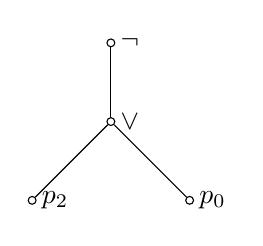
\begin{tikzpicture}
[level distance=1cm]
\tikzstyle{hollow node}=[circle,draw,inner sep=1]

\node(0)[hollow node]{} 
[sibling distance=20mm]
   child{node(1)[hollow node]{}
     child{node(2)[hollow node]{}}
     child{node(3)[hollow node]{}}};
   
\node[right]at(0){$\neg$};
\node[right]at(1){$\vee$};
\node[right]at(2){$p_2$};
\node[right]at(3){$p_0$};
\end{tikzpicture}
&
(c) \quad
\begin{tikzpicture}
[level distance=1cm]
\tikzstyle{hollow node}=[circle,draw,inner sep=1]

\node(0)[hollow node]{} 
[sibling distance=20mm]
   child{node(1)[hollow node]{}
     child{node(3)[hollow node]{}
       child{node(5)[hollow node]{}
         child{node(7)[hollow node]{}
            child{node(9)[hollow node]{}}
            child{node(10)[hollow node]{}}}
         child{node(8)[hollow node]{}}}
       child{node(6)[hollow node]{}}}
     child{node(4)[hollow node]{}}}
   child{node(2)[hollow node]{}};
   
\node[right]at(9){{$p_0$}};
\node[right]at(10){{$p_1$}};
\node[right]at(7){{$\wedge$}};
\node[right]at(8){{$p_2$}};
\node[right]at(5){{$\wedge$}};
\node[right]at(6){{$p_4$}};
\node[right]at(3){{$\wedge$}};
\node[right]at(4){{$p_5$}};
\node[right]at(1){{$\wedge$}};
\node[right]at(2){{$p_6$}};
\node[right]at(0){{$\wedge$}};
\end{tikzpicture}
\end{tabular}
\end{center}
\end{exercise}

\begin{proof}[Solution]\
    \begin{enumerate}
        \item[(a)]\ $(\neg \bot)$
        \item[(b)]\ $(\neg (p_2 \vee p_0))$
        \item[(c)]\ $((((((p_0 \vee p_1)\vee p_2) \vee p_3) \vee p_4) \vee p_5) \vee p_6)$
    \end{enumerate}
\end{proof}

\ \\
\begin{exercise}
Please solve Exercise 3.2.1 in the textbook using the definition of subformulas in the slides:

List all the subformulas of the following formula.
%
\[
((\neg ( p_2 \rightarrow (p_1 \leftrightarrow p_0 ))) \vee ( p_2 \rightarrow \bot ))
\]
\end{exercise}

\begin{proof}[Solution]\
  $p_2, p_1, p_0, \bot, (p_1 \leftrightarrow p_0), ( p_2 \rightarrow \bot ), ( p_2 \rightarrow (p_1 \leftrightarrow p_0 )), (\neg ( p_2 \rightarrow (p_1 \leftrightarrow p_0 ))), ((\neg ( p_2 \rightarrow (p_1 \leftrightarrow p_0 ))) \vee ( p_2 \rightarrow \bot ))$  
\end{proof}

\ \\
\begin{exercise}
Please solve Exercise 3.2.6 in the textbook: 
(Since by definition $dom f = dom g = N_1$, you just need to show that, for each $\mu \in N_1$, $f (\mu) = g (\mu)$.)

Suppose $( N_1 , D_1 )$ and $( N_2 , D_2 )$ are planar trees. 
An \emph{isomorphism} from $( N_1 , D_1 )$ to $( N_2 , D_2 )$ is a bijection $f : N_1 \rightarrow N_2$ such that for every node $\mu \in N_1$, if $D_1 (\mu) = ( \nu_1 , \dots , \nu_n )$ then $D_2 ( f(\mu)) = ( f(\nu_1) , \dots , f(\nu_n) )$. 
We say that two planar trees are \emph{isomorphic} if there is an isomorphism from the first to the second. (Then isomorphism is an equivalence relation.) 

Prove: If $f$ and $g$ are two isomorphisms from $( N_1 , D_1 )$ to $( N_2 , D_2 )$ then $f = g$.

[If $(N_1,D_1)$ has height $n$, prove by induction on $k$ that for each $k$, the functions $f$ and $g$ agree on all nodes of height $n - k$ in $N_1$.]
\end{exercise}

\begin{proof}\ \\
    Let $h$ be the height of $( N_1 , D_1 )$, $\mu$ be an arbitrary node s.t. $\mu \in N_1$, $k$ be arbitrary natural number s.t. $k \le h$ and $h - k$ be the height of $\mu$.\\
    We use induction on $k$. Suppose $D_1(\mu)=(\nu_1,...,\nu_m)$
    \begin{itemize}
        \item[\textbf{BS}:]
            $k=0$\\
            Then, the height of $\mu$ is $k$. Then, $\mu$ is the root of $(N_1,D_1)$.\\
            Suppose $f(\mu)$ is not the root of $D_2$.\\
            Since $f$ is an isomophism.\\
            Then, there is $\nu_i$ s.t.:\\
            $\nu_i \in D_1$ and 
            $D_2(f(\nu_i))=(...,f(\mu),...)$.\\ 
            Since $f$ is an isomophism. $D_1(\nu_i)=(...,\mu,...)$ holds.\\
            Thus, there is a path from $\nu_i$ to $\mu$.
            But $\mu$ is the root of $(N_1,D_1)$. There is no path from anyone to it.\\
            Contradiction!\\
            Hence, $f(\mu)$ is the root of $D_2$.\\
            Similarly, $g(\mu)$ is the root of $D_2$.\\
            Thus, $f(\mu)=g(\mu)$.
        \item[\textbf{IH}:]
            If $f(\mu)=g(\mu)$ holds when $k<n$, then $f(\mu)=g(\mu)$ holds when $k=n$. That is if $f(\mu)=g(\mu)$ holds when the height of $\mu$ is greater than $h-n$, then $f(\mu)=g(\mu)$ holds when the height of $\mu$ equals to $h-n$.
        \item[\textbf{IS:}]
            Suppose that the height of $\mu$ is $h-n+1$. Then by IH, $f(\mu)=g(\mu)$ holds.\\
            Since $f$ and $g$ are two isomophisms from $( N_1 , D_1 )$ to $( N_2 , D_2 )$. We know that:\\ 
            $D_2 ( f(\mu)) = ( f(\nu_1) , \dots , f(\nu_m) )$\\
            $D_2 ( g(\mu)) = ( g(\nu_1) , \dots , g(\nu_m) )$\\
            Thus, $( f(\nu_1) , \dots , f(\nu_m) )=( g(\nu_1) , \dots , g(\nu_m) )$.\\
            Thus, $f(\nu_i)=g(\nu_i)$ holds for every $\nu_i \in D_1(\mu)$.\\
            Since $\nu_i$ has the height $h-n$. Then, for every $\mu \in N_1$, $f(\mu)=g(\mu)$ holds when $\mu$ has the height $h-n$.
            
            
    \end{itemize}
    
This finish the proof by induction.   
\end{proof}

%文档内容结束
\end{document}
